\documentclass{article}
\usepackage{tikz}
\usepackage{amsmath}
\usepackage[paperwidth=24cm,paperheight=16cm,margin=0.5cm]{geometry}
\pagestyle{empty}
\begin{document}
\centering
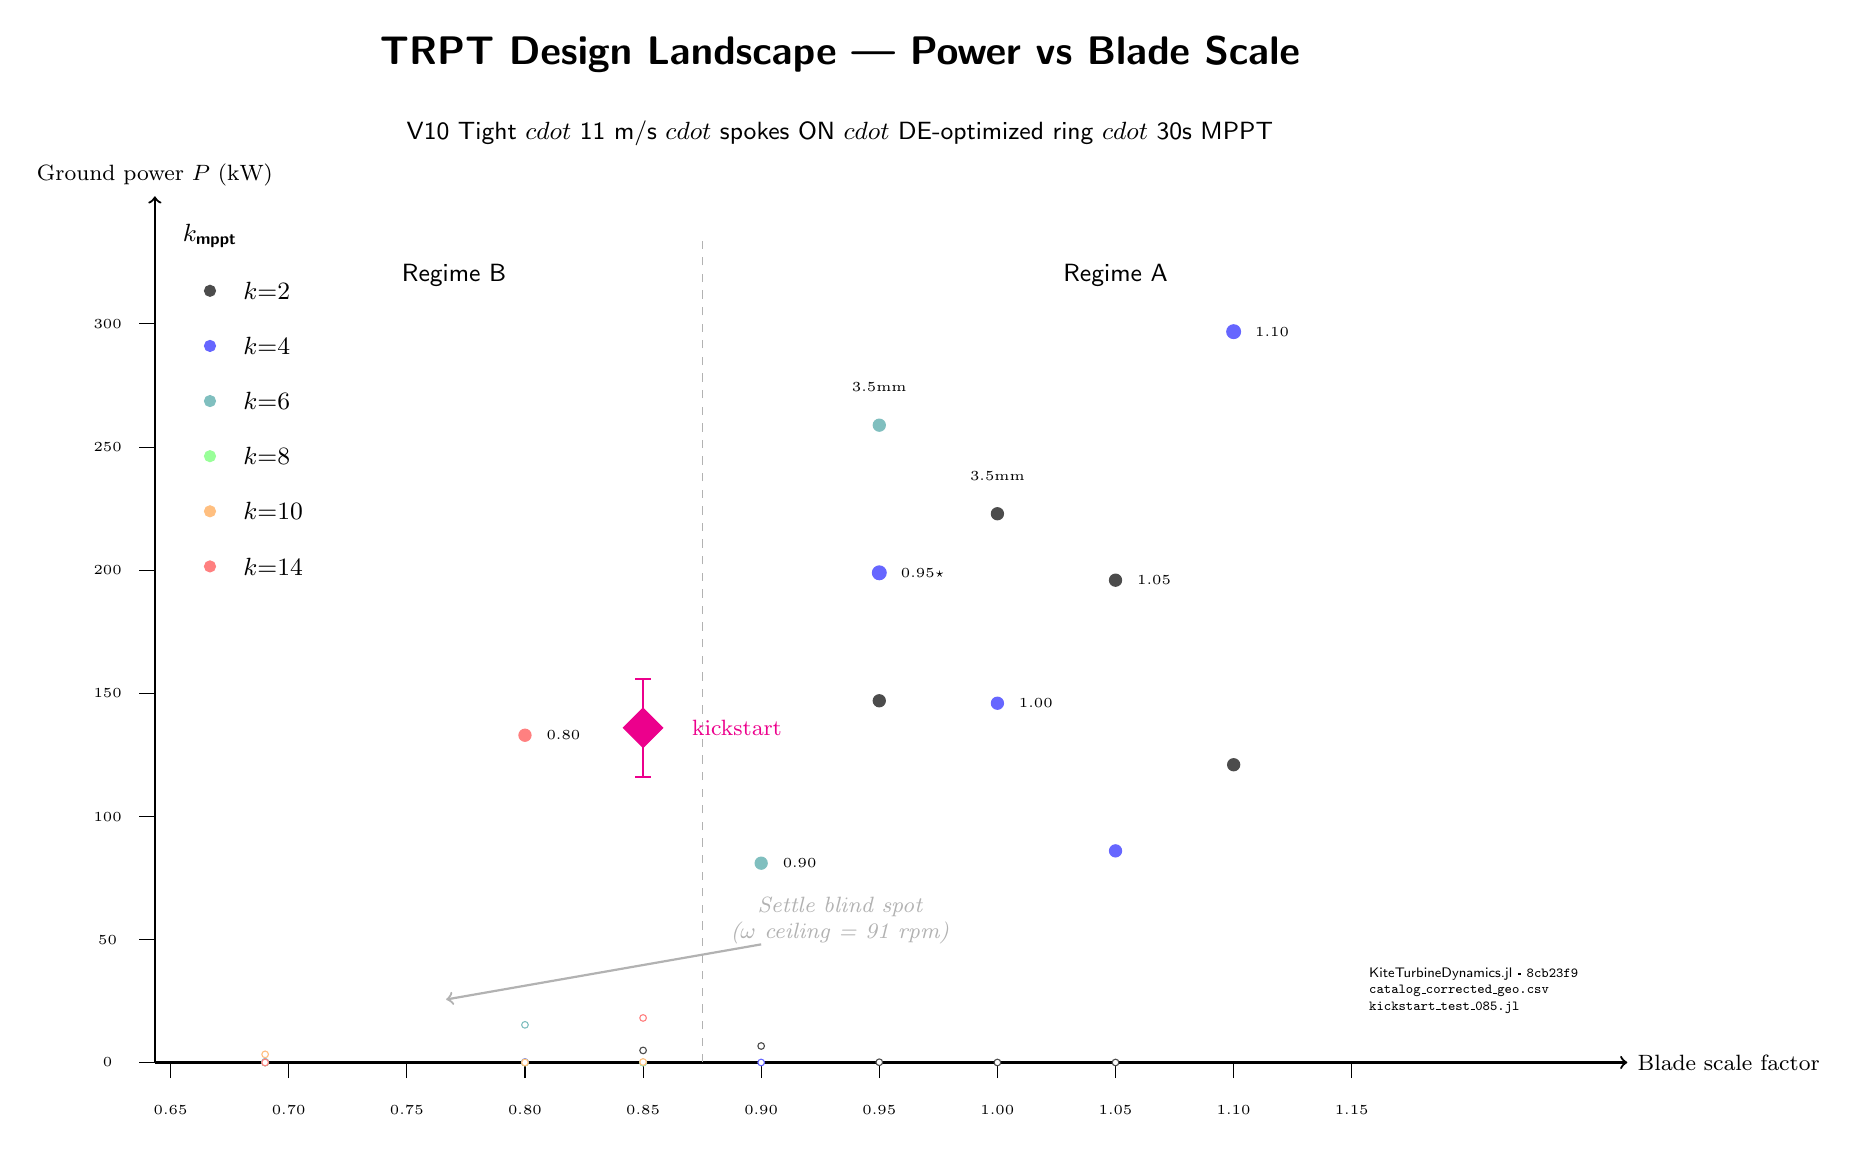
\begin{tikzpicture}[scale=1.0]

% ── Title ──
\node[font=\Large\sffamily\bfseries] at (10.5, 14.8) {TRPT Design Landscape — Power vs Blade Scale};
\node[font=\small\sffamily] at (10.5, 13.8) {V10 Tight $cdot$ 11 m/s $cdot$ spokes ON $cdot$ DE-optimized ring $cdot$ 30s MPPT};

% ── Axes ──
\draw[->, thick] (1.8, 2.0) -- (20.5, 2.0) node[right, font=\footnotesize] {Blade scale factor};
\draw[->, thick] (1.8, 2.0) -- (1.8, 13.0) node[above, font=\footnotesize] {Ground power $P$ (kW)};

% ── Tick marks X (blade_scale 0.65..1.15) ──
\foreach \b/\x in {0.65/2.0, 0.70/3.5, 0.75/5.0, 0.80/6.5, 0.85/8.0, 0.90/9.5, 0.95/11.0, 1.00/12.5, 1.05/14.0, 1.10/15.5, 1.15/17.0} {
  \draw (\x, 1.8) -- (\x, 2.0);
  \node[font=\tiny] at (\x, 1.4) {\b};
}

% ── Tick marks Y (0..320 kW) ──
\foreach \p/\y in {0/2.0, 50/3.56, 100/5.12, 150/6.69, 200/8.25, 250/9.81, 300/11.38} {
  \draw (1.6, \y) -- (1.8, \y);
  \node[font=\tiny] at (1.2, \y) {\p};
}

% ── Regime divider ──
\draw[dashed, gray!60] (8.75, 2.0) -- (8.75, 12.5);
\node[font=\small\sffamily, fill=white, fill opacity=0.92, text opacity=1] at (5.6, 12.0) {Regime B};
\node[font=\small\sffamily, fill=white, fill opacity=0.92, text opacity=1] at (14.0, 12.0) {Regime A};

% ── Helper macro for data points ──
% x = 2.0 + (blade - 0.65) * 30
% y = 2.0 + P / 32

% ── Failed points (open circles, small) ──
% blade 0.69: all k
\foreach \k/\p/\c in {2/0.0/black!70, 4/0.2/blue!60, 6/0.2/teal!50, 8/0.0/green!40, 10/3.3/orange!50, 14/0.0/red!50} {
  \pgfmathsetmacro{\px}{2.0 + (0.69-0.65)*30}
  \pgfmathsetmacro{\py}{2.0 + \p/32}
  \draw[\c, fill=white] (\px, \py) circle (1.2pt);
}
% blade 0.80: k=2,4,6,8,10
\foreach \k/\p/\c in {2/0.0/black!70, 4/0.2/blue!60, 6/15.3/teal!50, 8/0.0/green!40, 10/0.0/orange!50} {
  \pgfmathsetmacro{\px}{2.0 + (0.80-0.65)*30}
  \pgfmathsetmacro{\py}{2.0 + \p/32}
  \draw[\c, fill=white] (\px, \py) circle (1.2pt);
}
% blade 0.85: k=2,4,6,8,10,14
\foreach \k/\p/\c in {2/4.9/black!70, 4/0.0/blue!60, 6/0.0/teal!50, 8/0.0/green!40, 10/0.2/orange!50, 14/18.1/red!50} {
  \pgfmathsetmacro{\px}{2.0 + (0.85-0.65)*30}
  \pgfmathsetmacro{\py}{2.0 + \p/32}
  \draw[\c, fill=white] (\px, \py) circle (1.2pt);
}
% blade 0.90: k=2,4
\foreach \k/\p/\c in {2/6.7/black!70, 4/0.0/blue!60} {
  \pgfmathsetmacro{\px}{2.0 + (0.90-0.65)*30}
  \pgfmathsetmacro{\py}{2.0 + \p/32}
  \draw[\c, fill=white] (\px, \py) circle (1.2pt);
}
% blade 0.95: k=2
\pgfmathsetmacro{\px}{2.0 + (0.95-0.65)*30}
\pgfmathsetmacro{\py}{2.0 + 0.1/32}
\draw[black!70, fill=white] (\px, \py) circle (1.2pt);
% blade 1.00: k=2
\pgfmathsetmacro{\px}{2.0 + (1.00-0.65)*30}
\pgfmathsetmacro{\py}{2.0 + 0.0/32}
\draw[black!70, fill=white] (\px, \py) circle (1.2pt);
% blade 1.05: k=2
\pgfmathsetmacro{\px}{2.0 + (1.05-0.65)*30}
\pgfmathsetmacro{\py}{2.0 + 0.0/32}
\draw[black!70, fill=white] (\px, \py) circle (1.2pt);

% ── Viable points (filled circles, larger) ──
% blade 0.80, k=14, P=133
\pgfmathsetmacro{\px}{2.0 + (0.80-0.65)*30}
\pgfmathsetmacro{\py}{2.0 + 133/32}
\draw[red!50, fill=red!50] (\px, \py) circle (2.2pt);
\node[font=\tiny, right] at (\px+0.15, \py) {0.80};

% blade 0.90, k=6, P=81
\pgfmathsetmacro{\px}{2.0 + (0.90-0.65)*30}
\pgfmathsetmacro{\py}{2.0 + 81/32}
\draw[teal!50, fill=teal!50] (\px, \py) circle (2.2pt);
\node[font=\tiny, right] at (\px+0.15, \py) {0.90};

% blade 0.95, k=4, P=199
\pgfmathsetmacro{\px}{2.0 + (0.95-0.65)*30}
\pgfmathsetmacro{\py}{2.0 + 199/32}
\draw[blue!60, fill=blue!60] (\px, \py) circle (2.5pt);
\node[font=\tiny, right] at (\px+0.15, \py) {0.95\textbf{$\star$}};

% blade 0.95, k=6/3.5mm, P=259
\pgfmathsetmacro{\px}{2.0 + (0.95-0.65)*30}
\pgfmathsetmacro{\py}{2.0 + 259/32}
\draw[teal!50, fill=teal!50] (\px, \py) circle (2.2pt);
\node[font=\tiny, above] at (\px, \py+0.3) {3.5mm};

% blade 0.95, k=2/r1.0, P=147
\pgfmathsetmacro{\px}{2.0 + (0.95-0.65)*30}
\pgfmathsetmacro{\py}{2.0 + 147/32}
\draw[black!70, fill=black!70] (\px, \py) circle (2.2pt);

% blade 1.00, k=4, P=146
\pgfmathsetmacro{\px}{2.0 + (1.00-0.65)*30}
\pgfmathsetmacro{\py}{2.0 + 146/32}
\draw[blue!60, fill=blue!60] (\px, \py) circle (2.2pt);
\node[font=\tiny, right] at (\px+0.15, \py) {1.00};

% blade 1.00, k=2/3.5mm, P=223
\pgfmathsetmacro{\px}{2.0 + (1.00-0.65)*30}
\pgfmathsetmacro{\py}{2.0 + 223/32}
\draw[black!70, fill=black!70] (\px, \py) circle (2.2pt);
\node[font=\tiny, above] at (\px, \py+0.3) {3.5mm};

% blade 1.05, k=4, P=86
\pgfmathsetmacro{\px}{2.0 + (1.05-0.65)*30}
\pgfmathsetmacro{\py}{2.0 + 86/32}
\draw[blue!60, fill=blue!60] (\px, \py) circle (2.2pt);

% blade 1.05, k=2/r1.0, P=196
\pgfmathsetmacro{\px}{2.0 + (1.05-0.65)*30}
\pgfmathsetmacro{\py}{2.0 + 196/32}
\draw[black!70, fill=black!70] (\px, \py) circle (2.2pt);
\node[font=\tiny, right] at (\px+0.15, \py) {1.05};

% blade 1.10, k=4, P=297
\pgfmathsetmacro{\px}{2.0 + (1.10-0.65)*30}
\pgfmathsetmacro{\py}{2.0 + 297/32}
\draw[blue!60, fill=blue!60] (\px, \py) circle (2.5pt);
\node[font=\tiny, right] at (\px+0.15, \py) {1.10};

% blade 1.10, k=2/3.5mm, P=121
\pgfmathsetmacro{\px}{2.0 + (1.10-0.65)*30}
\pgfmathsetmacro{\py}{2.0 + 121/32}
\draw[black!70, fill=black!70] (\px, \py) circle (2.2pt);

% ── Kickstart point (diamond) ──
\pgfmathsetmacro{\kx}{2.0 + (0.85-0.65)*30}
\pgfmathsetmacro{\kyhi}{2.0 + 156/32}
\pgfmathsetmacro{\kylo}{2.0 + 116/32}
\pgfmathsetmacro{\kymid}{2.0 + 136/32}
% Error bar
\draw[magenta, thick] (\kx, \kylo) -- (\kx, \kyhi);
\draw[magenta, thick] (\kx-0.1, \kylo) -- (\kx+0.1, \kylo);
\draw[magenta, thick] (\kx-0.1, \kyhi) -- (\kx+0.1, \kyhi);
% Diamond
\draw[magenta, fill=magenta] (\kx, \kymid) ++(0.25,0) -- ++(-0.25,0.25) -- ++(-0.25,-0.25) -- ++(0.25,-0.25) -- cycle;
\node[font=\footnotesize, magenta, right] at (\kx+0.5, \kymid) {kickstart};

% ── Settle blind spot callout ──
\draw[->, gray!60, thick] (9.5, 3.5) -- (5.5, 2.8);
\node[font=\footnotesize\itshape, gray!60, align=center] at (10.5, 3.8) {Settle blind spot\\($\omega$ ceiling = 91 rpm)};

% ── Legend ──
\node[font=\small\sffamily\bfseries] at (2.5, 12.5) {$k_{\text{mppt}}$};
\foreach \k/\c/\cy in {2/black!70/11.8, 4/blue!60/11.1, 6/teal!50/10.4, 8/green!40/9.7, 10/orange!50/9.0, 14/red!50/8.3} {
  \draw[\c, fill=\c] (2.5, \cy) circle (2pt);
  \node[font=\small, right] at (2.8, \cy) {$k{=}\k$};
}

% ── Data provenance box ──
\node[font=\tiny\sffamily, align=left, anchor=south east] at (20.0, 2.5) {
  KiteTurbineDynamics.jl · \texttt{8cb23f9}\\
  \texttt{catalog\_corrected\_geo.csv}\\
  \texttt{kickstart\_test\_085.jl}
};

\end{tikzpicture}
\end{document}
